% ------------------------------------------------------------------------------
% Apêndices
% ------------------------------------------------------------------------------

	\chapter{Como fazer citações}

		Você pode fazer uma citação de diversas formas. Se você quiser fazer uma citação entre parênteses, você pode fazer assim: \citep{milgram1969note}. Se você quiser mencionar o número da página, você pode fazer assim: \citep[p. 10]{deb2002fast}. Agora, se você quiser fazer uma citação onde o autor é parte da sentença, você pode fazer assim: \cite{maxwell1865viii} afirma que... Se você quiser fazer uma citação com mais de um autor, você pode fazer assim: \citep{van2019fantastic,maxwell1865viii}.
	
	\chapter{Como escrever equações}

		Um exemplo básico de equação:
		\begin{equation}
			\boldsymbol{\mathcal{F}}(\mathbf{r}, t) = \mathfrak{Re}\{\mathbf{F}(\mathbf{r})e^{j\omega t}\} \label{eq:2:fourier}
		\end{equation}

		Um exemplo sobre como escrever múltiplas equações e o uso de fonte cursiva nas letras:
		\begin{eqnarray}
			\nabla\times\boldsymbol{\mathcal{E}}(\mathbf{r}, t) &=& - \frac{\partial\boldsymbol{ \mathcal{B}}}{\partial t}(\mathbf{r}, t) \label{eq:2:maxwell:time:1} \\
			\nabla\times\boldsymbol{\mathcal{H}}(\mathbf{r}, t) &=& \frac{\partial\boldsymbol{ \mathcal{D}}}{\partial t}(\mathbf{r}, t) + \boldsymbol{\mathcal{J}}(\mathbf{r}, t) \label{eq:2:maxwell:time:2} \\
			\nabla\cdot\boldsymbol{\mathcal{D}}(\mathbf{r}, t) &=& \rho(\mathbf{r}, t) \label{eq:2:maxwell:time:3} \\
			\nabla\cdot\boldsymbol{\mathcal{B}}(\mathbf{r}, t) &=& 0 \label{eq:2:maxwell:time:4}
		\end{eqnarray}

		Um exemplo de desenvolvimento de equação:
		\begin{eqnarray}
			\nabla\times\mathbf{H}(\mathbf{r}) &=&  j\omega\epsilon_0\epsilon_r\mathbf{E}(\mathbf{r}) + \sigma(\mathbf{r})\mathbf{E}(\mathbf{r})+ \mathbf{J}_i(\mathbf{r}) \label{eq:2:complexmedia:1} \\
			 &=&  j\omega\epsilon_0\left(\epsilon_r(\mathbf{r}) -j\frac{\sigma(\mathbf{r})}{\omega\epsilon_0}\right)\mathbf{E}(\mathbf{r}) +  \mathbf{J}_i(\mathbf{r}) \label{eq:2:complexmedia:2} \\
			&=&  j\omega\epsilon(\mathbf{r})\mathbf{E}(\mathbf{r}) +  \mathbf{J}_i(\mathbf{r}) \label{eq:2:complexmedia:3}
		\end{eqnarray}

		Um exemplo de equação quebrada em mais de uma linha:
		\begin{multline}
			\chi(\brho)E_{z_i}(\brho) = J_{z_{eq}}(\brho) + \frac{jk_b^2}{4} \chi(\brho) \int_S dS^\prime J_0(k_b|\brho-\brhop|) J_{z_{eq}}(\brhop) \\ + \frac{jk_b^2}{4} \chi(\brho) \int_S dS^\prime Y_0(k_b|\brho-\brhop|) J_{z_{eq}}(\brhop)  \label{eq:2:2d:greendecomp:csie}
		\end{multline}

		Um exemplo de equação com somatórios e integrais:
		\begin{multline}
			\iint_D E_{z_s}(\theta,\phi) w^{(\theta)}_u(\theta) w^{(\phi)}_v(\phi) d\theta d\phi = \\ -\frac{jk_b^2}{4} \sum\limits_{i=1}^{N_I}\sum\limits_{j=1}^{N_J} \sum\limits_{p=1}^{N_P}\sum\limits_{q=1}^{N_Q}\sum\limits_{r=1}^{N_R} a_{ij} b_{pqr} \iint\limits_{D} \iint\limits_{S} d\theta d\phi dxdy~ \bigg[ G^D_{2D}(\theta,x,y) \\ f^{(x)}_i(x) f^{(y)}_j(y) g^{(x)}_{p}(x) g^{(y)}_{q}(y) g^{(\phi)}_r(\phi)w^{(\theta)}_u(\theta) w^{(\phi)}_v(\phi)  \bigg], \\ u = 1,\cdots, N_U,~ v = 1,\cdots,N_V \label{eq:3:discretization:6}
		\end{multline}

		Um exemplo de definição de matriz:
		\begin{equation}
			\boldsymbol{\bar{\Lambda}} = \begin{bmatrix}
																\Lambda_{11} & \Lambda_{12} & \cdots & \Lambda_{1N_V} \\
															   \Lambda_{21} & \Lambda_{22} & \cdots & \Lambda_{2N_V} \\
															   \vdots & \vdots & \vdots & \vdots \\
															   \Lambda_{u1} & \Lambda_{u2} & \cdots & \Lambda_{uN_V} \\
															   \vdots & \vdots & \vdots & \vdots \\
															   \Lambda_{N_U1} & \Lambda_{N_U2} & \cdots & \Lambda_{N_UN_V}
															  \end{bmatrix} \label{eq:discretization:9}
	   \end{equation}

	   Um exemplo de definição de casos:
	   \begin{equation}
		w_{uv} = \begin{cases}
						  1,& \mathrm{in} ~D_{uv}, \\
						  0,& \mathrm{outside}, ~D_{uv}
					  \end{cases} \label{eq:3:discretization:subdomain}
		\end{equation}

		Um exemplo para organização de três matrizes em uma mesma linha:
		\begin{align}
			\boldsymbol{\bar{\chi}} &=	\begin{bmatrix}
														 \chi_{11} & 0 & \cdots & 0 \\
														 0 & \chi_{12} & \cdots & 0 \\
														 \vdots & \vdots & \ddots & \vdots \\
														  0 & 0 & \cdots & \chi_{N_IN_J}
													 \end{bmatrix}
			&\boldsymbol{\bar{\beta}} &=	\begin{bmatrix}
																\beta_{11} & 0 & \cdots & 0 \\
																0 & \beta_{12} & \cdots & 0 \\
																\vdots & \vdots & \ddots & \vdots \\
																0 & 0 & \cdots & \beta_{N_IN_J}
															\end{bmatrix}
			&\mathbf{\bar{R}} &=	\begin{bmatrix}
													R_{11} & 0 & \cdots & 0 \\
													0 & R_{12} & \cdots & 0 \\
													\vdots & \vdots & \ddots & \vdots \\
													0 & 0 & \cdots & R_{N_IN_J}
												\end{bmatrix} \label{eq:3:discretization:collocation:18}
		\end{align}

		Note que você pode referenciar equações das seguintes formas:
		\begin{itemize}
			\item Quando ela estiver no meio da frase, você pode usar simplesmente o comando \verb|\eqref{}|. Por exemplo: ``...como mostrado em \eqref{eq:2:maxwell:time:1}, ...''
			\item Quando você estiver no início da frase, você pode escrever: ``A Eq. \eqref{eq:2:maxwell:time:1} mostra que...''
		\end{itemize}
	
	\chapter{Como inserir figuras}

		Um exemplo sobre como inserir figuras simples pode ser visto em \ref{fig:2:scattering}. Você pode referenciar figuras através do comando \verb|\ref{}| ou do comando \verb|\autoref{}|. O primeiro comando apenas referencia o número da figura, enquanto o segundo comando referencia o número da figura e o nome dela. Por exemplo, você pode escrever: ``...como mostrado na \autoref{fig:2:scattering}, ...''.
		\begin{figure}[!tb]
			\centering
			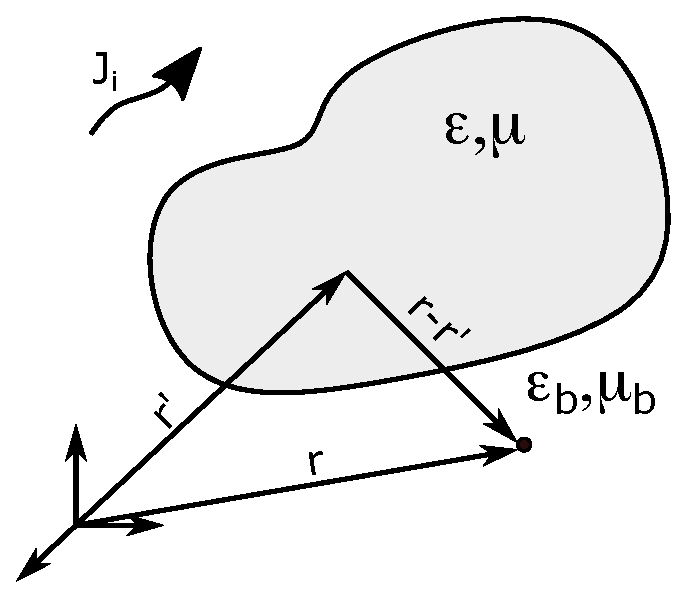
\includegraphics[width=0.5\textwidth]{./figuras/scattering}
			\caption{General scattering problem.}
			\label{fig:2:scattering}
		\end{figure}
	
	\chapter{Como inserir algoritmos}

		Um exemplo de algoritmo é o seguinte:
		\begin{algorithm}[!htb]
			\caption{Distorted Born Iterative Method.}
			\label{alg:dbim}
			\KwIn{$\mathbf{\bar{E}^s}$, $\mathbf{\bar{G}^{2D}}$, $\mathbf{\bar{G}^S}$}
			\KwOut{$\boldsymbol{\bar{\chi}}$, $\mathbf{\bar{E}}$}
			Compute an initial guess $\boldsymbol{\bar{\chi}^0}$ based on available information \\
			$t\leftarrow0$ \\
			\While{some criterion is not reached} {
				Solve $\left(\mathbf{\bar{I}} - \mathbf{\bar{G}^S}\boldsymbol{\bar{\chi}}^t\right)\mathbf{\bar{G}}^{\mathbf{in},t} = \mathbf{\bar{G}^{2D}}$ for $\mathbf{\bar{G}}^{\mathbf{in},t}$ \\
				Solve the direct problem for $\mathbf{\bar{E}}^t$ and $\mathbf{\bar{E}}^{\mathbf{s},t}$ \\
				$\Delta\mathbf{\bar{E}^s} = \mathbf{\bar{E}}^s - \mathbf{\bar{E}}^{\mathbf{s},t}$ \\
				Solve the inverse linear problem $\Delta\mathbf{\bar{E}^s} = \mathbf{\bar{G}}^{\mathbf{in},t}\Delta\boldsymbol{\bar{\chi}}\mathbf{\bar{E}}^t$ for $\Delta\boldsymbol{\bar{\chi}}$\\
				$\boldsymbol{\bar{\chi}}^t \leftarrow \boldsymbol{\bar{\chi}}^{t-1} + \Delta\boldsymbol{\bar{\chi}}^t$ \\
				$t\leftarrow t+1$\\
			}
		\end{algorithm}
	
	\chapter{Como inserir definições e outras coisas especiais}

		Um exemplo de definição:
		\begin{definition}\label{def:3:projection}
			Projection Operator\\
			Let $X$ be a normed space over the field $\mathbb{K}=\mathbb{R}$ or $\mathbb{K}=\mathbb{C}$. Let $U\subset X$ be a closed subspace. A linear bounded operator $\mathcal{P} : X\rightarrow X$ is called a projection operator on $U$ if
			\begin{itemize}
				\item $\mathcal{P}\{x\} \in U, ~\forall x\in X$ and
				\item $\mathcal{P}\{x\} = x,~ \forall x\in U$.
			\end{itemize}
		\end{definition}

	\chapter{Dyadic Green's Function}\label{app:green}
	
		The dyadic Green's function is an important tool for solving electromagnetic problems that include the radiation phenomenon. For this reason, this appendix aims to briefly discuss its definition and singularity. This text is based on chapter 7 of the book written by \cite{chew1995}, which deepens the discussion and provides a better bibliographical reference on the topic.
		%A função diádica de Green é uma importante ferramenta para a solução de problemas eletromagnéticos que incluem o fenômeno da radiação. Por isso, este apêndice tem o objetivo de fazer uma breve discussão sobre sua definição e valores singulares. Esse texto é baseado no capítulo 7 do livro escrito por \cite{chew1995}, o qual aprofunda a discussão do tema e traz uma referência bibliográfica mais completa sobre tema.

		\section{Dyadic Green's Function for Homogeneous Medium}\label{app:green:1}

			%Um problema muito comum e importante para a teoria eletromagnética é o de radiação de uma fonte pontual. Este problema é fundamental para equações integrais dado que a radiação de uma distribuição de corrente é baseado na contribuição de todos os pontos em que a corrente está definida. Isto é, considerando um problema escalar genérico como:
			A very general and essential problem for electromagnetic theory is that of radiation from a point source. This problem is fundamental for integral equations since the radiation of a current distribution is based on the contribution of all points at which the current is defined. That is, considering a generic scalar problem such as:
			\begin{equation}
				(\nabla^2+k^2)\phi(\mathbf{r}) = s(\mathbf{r}) \label{eq:app:green:1}
			\end{equation}

			%\noindent definida numa região homogênea $V$, a solução pode ser obtida através de:
			\noindent defined in a homogeneous region $V$, the solution can be obtained through:
			\begin{equation}
				\psi(\mathbf{r}) = - \int_V d\mathbf{r^\prime} g(\mathbf{r}, \mathbf{r^\prime})s(\mathbf{r^\prime}) \label{eq:app:green:2}
			\end{equation}

			%\noindent onde $g(\mathbf{r}, \mathbf{r^\prime})$ é a função de Green que é a solução para equação:
			\noindent where $g(\mathbf{r}, \mathbf{r^\prime})$ is the Green's function which is the solution to the equation:
			\begin{equation}
					(\nabla^2+k^2)g(\mathbf{r},\mathbf{r^\prime}) = -\delta(\mathbf{r}-\mathbf{r^\prime}) \label{eq:app:green:3}
			\end{equation}
	
			%Em outras palavras, essa solução decorre da interpretação que $s(\mathbf{r})$ é uma superposição linear de fontes pontuais.
			Particularly, this solution follows from the interpretation that $s(\mathbf{r})$ is a linear superposition of point sources.

			%Para obtermos a função de Green para um meio homogêneo e infinito, mudaremos a posição da fonte no prolema da eq.\eqref{eq:app:green:3} para a origem de coordenadas esféricas:
			To obtain Green's function for a homogeneous and infinite medium, we will change the source position in the problem of eq.\eqref{eq:app:green:3} to the origin of spherical coordinates:
			\begin{equation}
				(\nabla^2+k^2)g(\mathbf{r}) = -\delta(\mathbf{r}) = -\delta(x)\delta(y)\delta(z) \label{eq:app:green:4}
			\end{equation}
		
			%Para $\mathbf{r}\neq0$, a solução de \eqref{eq:app:green:4} é dado por:
			For $\mathbf{r}\neq0$, the solution of \eqref{eq:app:green:4} is given by:
			\begin{equation}
				g(\mathbf{r}) = C\frac{e^{jkr}}{r} + D\frac{e^{-jkr}}{r} \label{eq:app:green:5}
				\end{equation}
   
   			%\noindent onde $r = |\mathbf{r}|$. Pressupondo que não existem fontes no infinito, apenas o primeiro termo do lado direito de \eqref{eq:app:green:5} é solução:
   			\noindent where $r = |\mathbf{r}|$. Assuming that there are no sources at infinity, only the first term on the right-hand side of \eqref{eq:app:green:5} is a solution:
   			\begin{equation}
   				g(\mathbf{r}) = C\frac{e^{jkr}}{r} \label{eq:app:green:6}
   			\end{equation}

			%A constante $C$ é determinada ao calcularmos ambos os lados de \eqref{eq:app:green:4} na singularidade. Para fazermos isso, nós combinados \eqref{eq:app:green:6} em \eqref{eq:app:green:4} e integramos em um pequeno volume ao redor da origem:
			The constant $C$ is determined by calculating both sides of \eqref{eq:app:green:4} in the singularity. To do this, we combine \eqref{eq:app:green:6} into \eqref{eq:app:green:4} and integrated into a small volume around the origin:
			\begin{equation}
				\int_{\Delta V} dV \nabla\cdot\nabla\frac{Ce^{jkr}}{r} + \int_{\Delta V} dVk^2\frac{Ce^{jkr}}{r} = -1 \label{eq:app:green:7}
			\end{equation}
   
   			%A segunda integral de \eqref{eq:app:green:7} tende a zero se $\Delta V \rightarrow 0$, uma vez que $dV = 4\pi r^2dr$. Além disso, o teorema de Gauss pode ser utilizado para transformar a primeira integral em uma de superfície, e com isso, obtermos:
   			The second integral of \eqref{eq:app:green:7} tends to zero if $\Delta V \rightarrow 0$, since $dV = 4\pi r^2dr$. Besides, Gauss' theorem can be used to transform the first integral into a surface one, and with that, we obtain:
   			\begin{equation}
   				\lim\limits_{r\rightarrow0} 4\pi r^2\frac{d}{dr}C\frac{e^{jkr}}{r} = -1 \label{eq:app:green:8}
   			\end{equation} 

			%\noindent or $C=1/4\pi$. Além disso, a solução \eqref{eq:app:green:6} pode ser generalizado para o caso da fonte posicionada num ponto $\mathbf{r^\prime}$. Neste caso, a eq.\eqref{eq:app:green:6} pode ser reescrita como:
			\noindent or $C=1/4\pi$. Also, the solution \eqref{eq:app:green:6} can be generalized for the case in which the source is shifted to a point $\mathbf{r^\prime}$. In this case, eq.\eqref{eq:app:green:6} can be rewritten as:
			\begin{equation}
				g(\mathbf{r},\mathbf{r^\prime}) = g(\mathbf{r}-\mathbf{r^\prime}) = \frac{e^{jk|\mathbf{r}-\mathbf{r^\prime}|}}{4\pi |\mathbf{r}-\mathbf{r^\prime}|} \label{eq:app:green:9}
			\end{equation}
	
			%A solução \eqref{eq:app:green:6} pode ser utilizada para obtermos a função diádica\footnote{Dyads é um exemplo de um tensor de segundo rank, formado a partir de dois vetores e que mapeia um campo vetorial em um outro. Além disso, possuem a propriedade de terem espaço nulo de rank dois. Para um discussão mais profunda sobre tensores e suas propriedades matemáticas, recomendamos a leitura do Anexo B de \citep{chew1995}.} de Green para a equação vetorial de onda em um meio homogêneo e isotrópico:
			Solution (32) can be used to obtain Green's dyadic\footnote{Dyad is an example of a second rank tensor, formed from two vectors and maps one vector field to another. Besides, they have the property of having nullspace of rank two. For a deeper discussion of tensors and their mathematical properties, we recommend reading Appendix B of \citep{chew1995}.} function for the vector wave equation in a homogeneous and isotropic medium:
			\begin{equation}
				\nabla\times\nabla\times\mathbf{E}(\mathbf{r})-k^2\mathbf{E}(\mathbf{r}) = -j\omega\mu\mathbf{J}(\mathbf{r}) \label{eq:app:green:10}
			\end{equation}
	
			%Uma vez que $\nabla\times\nabla\times\mathbf{E} = -\nabla^2\mathbf{E} + \nabla\nabla\cdot\mathbf{E}$ e que, conforme a equação de continuidade, $\nabla\cdot\mathbf{E} = \varrho/\epsilon = \nabla\cdot\mathbf{J}/j\omega\epsilon$, a eq.\eqref{eq:app:green:10} pode ser reescrita como:
			Since $\nabla\times\nabla\times\mathbf{E} = -\nabla^2\mathbf{E} + \nabla\nabla\cdot\mathbf{E}$ and that, according to the continuity equation, $\nabla\cdot\mathbf{E} = \varrho/\epsilon = \nabla\cdot\mathbf{J}/j\omega\epsilon$, eq.\eqref{eq:app:green:10} can be rewritten as:
			\begin{equation}
				\nabla^2\mathbf{E}(\mathbf{r}) + k^2\mathbf{E}(\mathbf{r}) = j\omega\mu\left[\mathbf{\bar{I}}+\frac{\nabla\nabla}{k^2}\right]\cdot\mathbf{J}(\mathbf{r}) \label{eq:app:green:11}
			\end{equation}
	
			%\noindent onde $\mathbf{\bar{I}}$ é o operador identidade. Em coordenadas cartesianas, a eq.\eqref{eq:app:green:11} é na verdade três equações as quais podem ser resolvidas tal qual foi feito para a equação escalar. Desta forma, a solução para \eqref{eq:app:green:11} é:
			\noindent where $\mathbf{\bar{I}}$ is the identity operator. In Cartesian coordinates, eq.\eqref{eq:app:green:11} is actually three equations that can be solved just as it was done for the scalar equation. Thus, the solution for \eqref{eq:app:green:11} is:
			\begin{equation}
				\mathbf{E}(\mathbf{r}) = -j\omega\mu\int_V d\mathbf{r^\prime} g(\mathbf{r^\prime}-\mathbf{r})\left[\mathbf{\bar{I}}+\frac{\nabla^\prime\nabla^\prime}{k^2}\right]\cdot\mathbf{J}(\mathbf{r^\prime}) \label{eq:app:green:12}
			\end{equation}
	
			%Levando em consideração as identidades vetoriais $\nabla gf = f\nabla g + g\nabla f$ e $\nabla\cdot g\mathbf{F} = g\nabla\cdot\mathbf{F} + (\nabla g)\cdot\mathbf{F}$, as seguintes integrais podem ser reescritas como:
			Taking into account the vector identities $\nabla gf = f\nabla g + g\nabla f$ and $\nabla\cdot g\mathbf{F} = g\nabla\cdot\mathbf{F} + (\nabla g)\cdot\mathbf{F}$, the following integrals can be rewritten as:
			\begin{eqnarray}
				\int_V d\mathbf{r^\prime} g(\mathbf{r^\prime}-\mathbf{r})\nabla^\prime f(\mathbf{r^\prime}) &=& - \int_V \left[\nabla^\prime g(\mathbf{r^\prime}-\mathbf{r})\right]f(\mathbf{r^\prime}) \label{eq:app:green:13} \\
				 \int_V d\mathbf{r^\prime} \left[\nabla^\prime g(\mathbf{r^\prime}-\mathbf{r})\right]\nabla^\prime\cdot\mathbf{J}(\mathbf{r^\prime}) &=& -\int_V d\mathbf{r}^\prime\mathbf{J}(\mathbf{r^\prime})\cdot\nabla^\prime\nabla^\prime g(\mathbf{r^\prime}-\mathbf{r}) \label{eq:app:green:14}
			\end{eqnarray}
	
			%\noindent o que permite reescrever \eqref{eq:app:green:12} como:
			\noindent which allows us to rewrite \eqref{eq:app:green:12} as:
			\begin{equation}
				\mathbf{E}(\mathbf{r}) = -j\omega\mu\int_V d\mathbf{r^\prime} \mathbf{J}(\mathbf{r^\prime})\cdot\left[\mathbf{\bar{I}}+\frac{\nabla^\prime\nabla^\prime}{k^2}\right]g(\mathbf{r^\prime},\mathbf{r}) \label{eq:app:green:15}
			\end{equation}
		
			%No entanto, conforme demonstrado no capítulo 7 de \citep{chew1995}, também é possível escrever a eq.\eqref{eq:app:green:15} da seguinte forma:
			However, as demonstrated in chapter 7 of \citep{chew1995}, it is also possible to write eq.\eqref{eq:app:green:15} as follows:
			\begin{equation}
				\mathbf{E}(\mathbf{r}) = j\omega\mu\int_V d\mathbf{r^\prime} \mathbf{J}(\mathbf{r^\prime})\cdot\mathbf{\bar{G}}(\mathbf{r},\mathbf{r^\prime}) \label{eq:app:green:16}
			\end{equation}
		
			%\noindent onde:
			\noindent where:
			\begin{equation}
				\mathbf{\bar{G}}(\mathbf{r},\mathbf{r^\prime}) = -\left[\mathbf{\bar{I}}+\frac{\nabla\nabla}{k^2}\right]\frac{e^{jk|\mathbf{\mathbf{r}-\mathbf{r^\prime}}|}}{4\pi|\mathbf{\mathbf{r}-\mathbf{r^\prime}}|} \label{eq:app:green:17}
			\end{equation}
		
		\section{The Singularity of the Dyadic Green's Function}\label{app:green:2}
		
			%Conforme pode ser observado na equação \eqref{eq:app:green:13}, a função diádica de Green tem singularidade para $\mathbf{r}=\mathbf{r^\prime}$. Ou seja, para calcular o campo em um ponto dentro da região da fonte $\mathbf{J}$, é necessário reescrever a equação integral \eqref{eq:app:green:16} com o suporte do volume de exclusão $V_\delta$ em torno do ponto de singularidade:
			As can be seen in equation \eqref{eq:app:green:13}, Green's dyadic function has singularity for $\mathbf{r}=\mathbf{r^\prime}$. That is, to calculate the field at a point within the region of the source $\mathbf{J}$, it is necessary to rewrite the integral equation \eqref{eq:app:green:16} with the support of the exclusion volume $V_\delta$ around the singularity point:
			\begin{equation}
				\mathbf{E}(\mathbf{r}) = \lim\limits_{V_\delta\rightarrow0} j\omega\mu\int\limits_{V-V_\delta} d\mathbf{r^\prime} \mathbf{J}(\mathbf{r^\prime})\cdot\mathbf{\bar{G}}(\mathbf{r^\prime},\mathbf{r}) \label{eq:app:green:18}
			\end{equation}
		
			%Desta forma, a equação é definida em termos de uma integral imprópria. Geralmente, as integrais impróprias convergem se existir um limite fixo independente da forma de $V_\delta$. No entanto, no caso de \eqref{eq:app:green:18}, uma condição necessária para que integral convirja é que $\mathbf{J}$ satisfaça a condição de Holder \citep{kellogg1953foundations} em $\mathbf{r}=\mathbf{r^\prime}$, na qual deve haver constantes $c$, $A$ e $\alpha$ tal que $|\mathbf{J}(\mathbf{r})-\mathbf{J}(\mathbf{r^\prime})\le A|\mathbf{r^\prime}-\mathbf{r}|^{\alpha}$ para $|\mathbf{r^\prime}-\mathbf{r}| < c$. Essa condição é ligeiramente mais forte que continuidade normal. Além disso, as derivadas de \eqref{eq:app:green:17} não permitem que a integral convirja de maneira tradicional, i.e., o valor principal da integral existe mas depende da forma escolhida para $V_\delta$.
			In this way, the equation is defined in terms of an improper integral. Generally, improper integrals converge if there is a fixed limit regardless the shape of $V_\delta$. However, in the case of \eqref{eq:app:green:18}, a necessary condition for convergence is that $\mathbf{J}$ must satisfy Holder's condition \citep{kellogg1953foundations} in $\mathbf{r}=\mathbf{r^\prime}$, in which there must be constants $c$, $A$, and $\alpha$ such that $|\mathbf{J}(\mathbf{r})-\mathbf{J}(\mathbf{r^\prime})\le A|\mathbf{r^\prime}-\mathbf{r}|^{\alpha}$ for $|\mathbf{r^\prime}-\mathbf{r}| < c$. This condition is slightly stronger than general continuity. In addition, the derivatives of \eqref{eq:app:green:17} do not allow the integral to converge in a traditional fashion, i.e., the principal value of the integral exists but depends on the chosen shape for $V_\delta$.
			
			%Para cacularmos o limite do termo que inclui as derivadas na eq.\eqref{eq:app:green:18}, precisamos levar em consideração tanto a integral sobre a região sem a singularidade como a região com a singularidade:
			To calculate the limit of the term that includes those derived in eq.\eqref{eq:app:green:18}, we need to take into account both the integral over the region without the singularity and the region with the singularity:
			\begin{eqnarray}
				\nabla\nabla\cdot\int_V d\mathbf{r^\prime} g(\mathbf{r},\mathbf{r^\prime})\mathbf{J}(\mathbf{r^\prime}) &=& \lim\limits_{V_\delta\rightarrow0} \left[\nabla\nabla\cdot\int\limits_{V-V_\delta} d\mathbf{r^\prime} g(\mathbf{r},\mathbf{r^\prime})\mathbf{J}(\mathbf{r^\prime})\right.\nonumber \\ &&\left.~~~~~~~~~~~~~+~\nabla\nabla\cdot\int\limits_{V_\delta} d\mathbf{r^\prime} g(\mathbf{r},\mathbf{r^\prime})\mathbf{J}(\mathbf{r^\prime})\right] \label{eq:app:green:19}
			\end{eqnarray}
		
			%\noindent onde $\mathbf{r}\in V_{\delta}$. A primeira integral do lado direito da integral não contém $\mathbf{r}$, por isso, o operador $\nabla\nabla\cdot$ pode entrar na integral. Já a segunda integral converge somente se um operador $\nabla$ for introduzido na integral. Desta forma, a eq.\eqref{eq:app:green:19} pode ser reescrita como:
			\noindent where $\mathbf{r}\in V_{\delta}$. The first integral on the right-hand side of the equation does not contain $\mathbf{r}$, so the operator $\nabla\nabla\cdot$ might enter into the integral. The second integral converges only if an operator $\nabla$ is introduced in the integral. In this way, eq.\eqref{eq:app:green:19} can be rewritten as:
			\begin{eqnarray}
				\nabla\nabla\cdot\int_V d\mathbf{r^\prime} g(\mathbf{r},\mathbf{r^\prime})\mathbf{J}(\mathbf{r^\prime}) &=& \lim\limits_{V_\delta\rightarrow0} \left[\int\limits_{V-V_\delta} d\mathbf{r^\prime} \nabla\nabla\cdot g(\mathbf{r},\mathbf{r^\prime})\mathbf{J}(\mathbf{r^\prime})\right.\nonumber \\ &&\left.~~~~~~~~~~~~~-~\nabla\int\limits_{V_\delta} d\mathbf{r^\prime} \nabla^\prime g(\mathbf{r},\mathbf{r^\prime})\cdot\mathbf{J}(\mathbf{r^\prime})\right] \label{eq:app:green:20}
			\end{eqnarray}
		
			%Portanto, as duas integrais no lado direito de \eqref{eq:app:green:20} convergem a um valor que depende da forma de $V_\delta$. No entanto, a soma das duas integrais tem que ser igual ao lado esquerdo o qual independe da forma escolhida para $V_\delta$. 
			Therefore, the two integrals on the right-hand side of \eqref{eq:app:green:20} converge to a value that depends on the shape of $V_\delta$. However, the sum of the two integrals must be equal to the left-hand side, which does not depend on the shape chosen for $V_\delta$.
			
			%Se utilizarmos a integração por partes e utilizarmos a relação $\nabla\cdot\mathbf{J}=j\omega\varrho$, a segunda integral de \eqref{eq:app:green:20} pode ser reescrita como:
			If we use the integration by parts and the relation $\nabla\cdot\mathbf{J}=j\omega\varrho$, the second integral of (46) can be rewritten as:
			\begin{eqnarray}
				\nabla\int\limits_{V_\delta} d\mathbf{r^\prime} \nabla^\prime g(\mathbf{r},\mathbf{r^\prime})\cdot\mathbf{J}(\mathbf{r^\prime}) = \int_{S_\delta} dS^\prime \mathbf{n}\cdot\mathbf{J}(\mathbf{r^\prime})g(\mathbf{r},\mathbf{r^\prime}) - j\omega\int_{V_\delta} g(\mathbf{r},\mathbf{r^\prime})\varrho(\mathbf{r^\prime}) \label{eq:app:green:21}
			\end{eqnarray}
		
			%A segunda integral de \eqref{eq:app:green:21} tenderá a zero quando $V_\delta\rightarrow0$ assumindo que, para uma corrente volumétrica, $\varrho(\mathbf{r})$ é contínua. Já a primeira integral tem o termo $\mathbf{n}\cdot\mathbf{J}(\mathbf{r^\prime})$ o qual é a carga superficial em $S_{\delta}$, a superfície de $V_\delta$. Por causa dessa carga superficial, a primeira integral é proporcional ao campo em $\mathbf{r}$ e não varia conforme a escala. Em outras palavras, ela não desaparece quando $V_\delta\rightarrow0$, mas depende da forma de $V_\delta$. No limite, a eq.\eqref{eq:app:green:21} é linearmente proporcional a $\mathbf{J}(\mathbf{r})$. Portanto, com o auxílio de uma dyad $\mathbf{\bar{L}}$ dependente da forma de $V_\delta$, podemos reescrever \eqref{eq:app:green:20} como:
			The second integral of \eqref{eq:app:green:21} will tend to zero when $V_\delta\rightarrow0$ assuming that, for a volumetric current, $\varrho(\mathbf{r})$ is continuous. The first integral, on the other hand, has the term $\mathbf{n}\cdot\mathbf{J}(\mathbf{r^\prime})$ which is the surface charge on $S_{\delta}$, the surface of $V_\delta$. Because of this surface charge, the first integral is proportional to the field in $\mathbf{r}$ and does not vary depending on the scale. In other words, it does not disappear when $V_\delta\rightarrow0$, but depends on the shape of $V_\delta$. At the limit, eq.\eqref{eq:app:green:21} is linearly proportional to $\mathbf{J}(\mathbf{r})$. Therefore, with the aid of $\mathbf{\bar{L}}$, a dyad which depends on the shape of $V_\delta$, we can rewrite \eqref{eq:app:green:20} as:
			\begin{equation}
				\nabla\nabla\cdot\int_V d\mathbf{r^\prime} g(\mathbf{r},\mathbf{r^\prime})\mathbf{J}(\mathbf{r^\prime}) = \lim\limits_{V_\delta\rightarrow0}\int\limits_{V-V_\delta}d\mathbf{r^\prime}\nabla\nabla(\mathbf{r},\mathbf{r^\prime})\cdot\mathbf{J}(\mathbf{r^\prime})-\mathbf{\bar{L}}\cdot\mathbf{J}(\mathbf{r}) \label{eq:app:green:22}
			\end{equation}
		
			%Usando este resultado em \eqref{eq:app:green:16}, obteremos:
			Using this result in \eqref{eq:app:green:16}, we will obtain:
			\begin{equation}
				\mathbf{E}(\mathbf{r}) = j\omega\mu\lim\limits_{V_\delta\rightarrow0}\int\limits_{V-V_\delta}d\mathbf{r^\prime}\mathbf{\bar{G}}(\mathbf{r}, \mathbf{r^\prime})\cdot\mathbf{J}(\mathbf{r^\prime}) + \frac{\mathbf{\bar{L}}\cdot\mathbf{J}(\mathbf{r})}{j\omega\epsilon} \label{eq:app:green:23}
			\end{equation}
		
			%A integral de \eqref{eq:app:green:23} é equivalente ao operador de integral de valor principal cuja notação é expressa por $P.V.\int_V$, ou seja:
			The integral of \eqref{eq:app:green:23} is equivalent to the principal value integral operator whose notation is expressed by $P.V.\int_V$, that is:
			\begin{equation}
				\mathbf{E}(\mathbf{r}) = j\omega\mu P.V.\int_V d\mathbf{r^\prime}\mathbf{\bar{G}}(\mathbf{r}, \mathbf{r^\prime})\cdot\mathbf{J}(\mathbf{r^\prime}) + \frac{\mathbf{\bar{L}}\cdot\mathbf{J}(\mathbf{r})}{j\omega\epsilon},~~~\forall\mathbf{r}\in V \label{eq:app:green:24}
			\end{equation}
			
			%Portanto, embora os dois termos do lado direito de \eqref{eq:app:green:24} sejam dependentes da escolha de $V_\delta$, o campo $\mathbf{E}$ é único. Este método para determinar o valor campo na região de singularidade é conhecido como Método do Volume Principal \citep{vanbladel1961some}.
			Therefore, although the two terms on the right-hand side of \eqref{eq:app:green:24} are dependent on the choice of $V_\delta$, the $\mathbf{E}$ field is unique. This method for determining the field value in the region of singularity is known as the Principal Volume Method \citep{vanbladel1961some}.
			
			%Fisicamente, este método de solução corresponde a abrir um espaço ao redor do ponto de observação dentro região da corrente. Uma vez que essa corrente é discontínua na superfície desse espaço, a superfície acumula cargas as quais, ao diminuir o espaço para um volume infinitesimal, têm natureza eletrostática. Esse campo eletrostático satisfaz a equação de Laplace e está em função da forma desse espaço não importando qual pequeno ele seja. Portanto, o segundo termo da eq.\eqref{eq:app:green:24} tem o objetivo de remover a contribuição desse campo eletrostático, uma vez que ele não faz parte do problema mas foi adicionado como um recurso matemático.
			Physically, this method of solution corresponds to opening a space around the observation point within the current region. Since this current is discontinuous on the surface of that space, the surface accumulates charges which, when decreasing the space to an infinitesimal volume, have an electrostatic nature. This electrostatic field satisfies the Laplace equation and depends on the shape of that space, no matter how small it is. Therefore, the second term in eq.\eqref{eq:app:green:24} aims to remove the contribution from this electrostatic field, since it is not part of the problem but has been added as a mathematical resource.
			
			%Por fim, alguns valores de $\mathbf{\bar{L}}$ para determinados tipos de volumes de exclusão já foram determinados na literatura \citep{yaghjian1980electric, lee1980singularity}. Além disso, geralmente, o traço $\left[\mathbf{\bar{L}}\right] = 1$ \citep{yaghjian1980electric}. O quadro \ref{board:Lvalues} mostra alguns valores de $\mathbf{\bar{L}}$ para algumas formas geométricas:
			Finally, some values for $\mathbf{\bar{L}}$ for certain types of exclusion volumes have already been determined in the literature \citep{yaghjian1980electric, lee1980singularity}. In addition, generally, the trace $\left[\mathbf{\bar{L}}\right]=1$ \citep{yaghjian1980electric}. Board \ref{board:Lvalues} shows some values for $\mathbf{\bar{L}}$ considering some geometric shapes:
			
			\begin{table}[!htb]
				\centering
				\caption{Dyad $\mathbf{\bar{L}}$ values for different shapes of exclusion volume applied to the singularity of dyadic Green's function. Sources: \citep{yaghjian1980electric,lee1980singularity}.}
				\renewcommand{\arraystretch}{2.0}
				\begin{tabular}{cc}
					\textbf{Geometric shape} & $\mathbf{\bar{L}}$  \\\hline\hline
					Spheres or cubes & $\frac{\mathbf{\bar{I}}}{3}$ \\
					Disks & $\mathbf{z}\mathbf{z}$ \\
					Needles & $\frac{\mathbf{x}\mathbf{x}+\mathbf{y}\mathbf{y}}{2}$ \\
				\end{tabular}
				\label{board:Lvalues}
			\end{table}
			
		
		\section{Dyadic Green's Function for Inhomogeneous Medium}\label{app:green:3}
			
			%Para determinarmos a função diádica de Green para um meio não-homogêneo, vamos supor uma região $V_1$ e outra $V_2\subset V_1$. Os contrastes desses meios em relação ao vácuo serão denominados $\chi_{1}$ e $\chi_{2}$, respectivamente. Podemos escrever $\chi_{2}$ como:
			To determine the dyadic Green function for a non-homogeneous medium, we will assume a region $V_1$  and another $V_2\subset V_1$. The contrasts of these media in relation to the vacuum will be denominated $\chi_{1}$ and $\chi_{2}$, respectively. We can write $\chi_{2}$ as:
			\begin{equation}
				\chi_{2}(\mathbf{r}) = \chi_{1}(\mathbf{r}) + \Delta\chi(\mathbf{r}) \label{eq:app:green:25}
			\end{equation}
		
			%Deste modo, a equação integral para o campo elétrico em qualquer ponto do espaço pode ser escrita como:
			Consequently, the integral equation for the electric field at any point in space can be written as:
			\begin{equation}
				\mathbf{E}(\mathbf{r}) = \mathbf{E_i}(\mathbf{r}) + k_0^2\int_{V_1}d\mathbf{r^\prime}~\mathbf{\bar{G}}(\mathbf{r},\mathbf{r^\prime})\cdot\chi_1(\mathbf{r^\prime})\mathbf{E}(\mathbf{r^\prime}) + k_0^2\int_{V_1}d\mathbf{r^\prime}~\mathbf{\bar{G}}(\mathbf{r},\mathbf{r^\prime})\cdot\chi_2(\mathbf{r^\prime})\mathbf{E}(\mathbf{r^\prime}) \label{eq:app:green:26}
			\end{equation}
   
   			%No entanto, o campo $\mathbf{E}$ pode ser interpretado como a soma entre o campo espalhado causado pelo \textit{excesso} de contraste em $V_2$ quando o campo incidente é o campo que propaga num meio não-homogêneo caracterizado por $\epsilon_0$ para $\mathbf{r}\notin V_1$ e por $\chi_1$ para $\mathbf{r}\in V_1$. Matematicamente, isto equivale a:
   			However, $\mathbf{E}$ can be interpreted as the sum of the scattered field and by $\chi_1$ for $\mathbf{r}\in V_1$. The former is due to the \textit{excess} of contrast in $V_2$ when the incident field is the field that propagates in an inhomogeneous medium characterized by $\epsilon_0$ for $\mathbf{r}\notin V_1$. Mathematically, this is equivalent to:
   			\begin{equation}
   				\mathbf{E}(\mathbf{r}) = \mathbf{E_1}(\mathbf{r}) + k_0^2\int_{V_2} d\mathbf{r^\prime}~ \mathbf{\bar{G}_{in}}(\mathbf{r},\mathbf{r^\prime})\cdot\chi_2(\mathbf{r^\prime})\mathbf{E}(\mathbf{r^\prime}) \label{eq:app:green:27}
   			\end{equation}
   		
   			%\noindent onde $\mathbf{E_1}$ é dado por:
   			\noindent where $\mathbf{E_1}$ is given by:
   			\begin{equation}
   				\mathbf{E_1}(\mathbf{r}) = \mathbf{E_i}(\mathbf{r}) + k_0^2\int_{V_1} d\mathbf{r^\prime}~ \mathbf{\bar{G}}(\mathbf{r},\mathbf{r^\prime})\cdot\chi_1(\mathbf{r^\prime})\mathbf{E}(\mathbf{r^\prime}) \label{eq:app:green:28}
   			\end{equation}
   			
   			%\noindent e a função de Green para o meio não-homogêneo satisfaz:
   			\noindent and the Green's function for the inhomogeneous medium satisfies:
   			\begin{equation}
   				\mathbf{\bar{G}_{in}}(\mathbf{r},\mathbf{r^\prime}) = \mathbf{\bar{G}}(\mathbf{r},\mathbf{r^\prime}) + k_0^2 \int_{V_1}d\mathbf{r^{\prime\prime}} \mathbf{\bar{G}}(\mathbf{r},\mathbf{r^{\prime\prime}})\cdot\chi_{1}(\mathbf{r^{\prime\prime}})\mathbf{\bar{G}_{in}}(\mathbf{r^{\prime\prime}},\mathbf{r^\prime}) \label{eq:app:green:29}
   			\end{equation}
   		
   			%Soluções analíticas para \eqref{eq:app:green:29} são raramente disponíveis. Na maior parte das vezes em que uma modelagem não-homogenêa para a função de Green é necessária, métodos numéricos são empregados para estimar essa função.
   			Analytical solutions for \eqref{eq:app:green:29} are rarely available. Frequently, when inhomogeneous modeling for Green's function is necessary, numerical methods are employed to estimate this function.
   
    \chapter{Integral Equation Formulation}\label{app:integral}
    
   		Integral equations are an important method for electromagnetic theory. In this appendix, the derivation of the Electric Field Integral Equation from wave equation and dyadic Green's function will be discussed. The text is based on section 3.4 of \citep{chew2009}.

		Let us suppose a volume $V_ {inf}$ whose surface is $S_{inf}$ in which there is a source $J_2$ within a region $V_2$ and another source $J_1$ for a region $V_1$ separate from $V_2$ for a closed surface $S$ (see Figure \ref{fig:app:integral:integralequation}). Assuming that the medium in $V_1$ is homogeneous with properties $\epsilon_1$ and $\mu_1$, the relationship between electric field $\mathbf{E}(\mathbf{r}$) and a current distribution $\mathbf{J}(\mathbf{r}) $ representing currents $J_1$ and $J_2$ is given by the wave equation:
    	\begin{equation}
    		\nabla\times\nabla\times\mathbf{E}(\mathbf{r}) - \omega^2\epsilon_1\mu_1\mathbf{E}(\mathbf{r}) = -j\omega\mu_1\mathbf{J}(\mathbf{r}) \label{eq:app:integral:1}
   	 	\end{equation}
   	 	\begin{figure}[!htb]
			\centering
			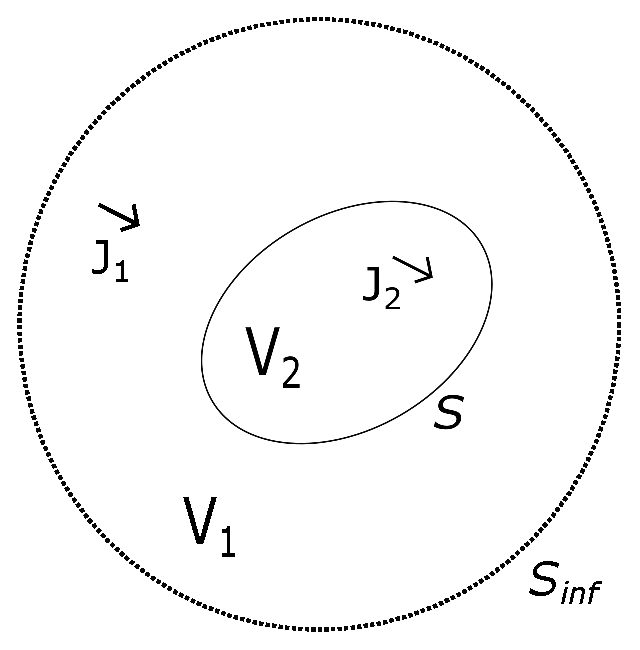
\includegraphics[width=0.4\textwidth]{./figuras/integralequation}
			\caption{Derivation of integral equation.}
			\label{fig:app:integral:integralequation}
		\end{figure}

		The solution to this equation is obtained with the support of the dyadic Green's function $\mathbf{\bar{G}}(\mathbf{r},\mathbf{r^\prime})$ for a homogeneous and isotropic medium, where $\mathbf{r^\prime}$ is an observation point in the source region. Under these conditions, the Green's function is a solution to the following equation:
		\begin{equation}
			\nabla\times\nabla\times\mathbf{\bar{G}}(\mathbf{r}, \mathbf{r^\prime}) - \omega^2\epsilon_1\mu_1\mathbf{\bar{G}}(\mathbf{r}, \mathbf{r^\prime}) = -\mathbf{\bar{I}}\delta(\mathbf{r}-\mathbf{r^\prime}) \label{eq:app:integral:2}
		\end{equation}

		Postmultiplying \eqref{eq:app:integral:1} by $\mathbf{\bar{G}}(\mathbf{r}, \mathbf{r^\prime})$, premultiplying \eqref{eq:app:integral:2} by $\mathbf{E}(\mathbf{r})$, and then subtracting the resultant equations, we will obtain:
		\begin{eqnarray}
			\mathbf{E}(\mathbf{r})\cdot\nabla\times\nabla\times\mathbf{\bar{G}}(\mathbf{r},\mathbf{r^\prime}) - 	\nabla\times\nabla\times\mathbf{E}(\mathbf{r})\cdot\mathbf{\bar{G}}(\mathbf{r},\mathbf{r^\prime}) \nonumber \\ = j\omega\mu_1\mathbf{J}(\mathbf{r})\cdot\mathbf{\bar{G}}(\mathbf{r},\mathbf{r^\prime}) - \mathbf{E}(\mathbf{r})\delta(\mathbf{r}-\mathbf{r^\prime}) \label{eq:app:integral:4}
		\end{eqnarray}

		If we integrate both sides of the equation \eqref{eq:app:integral:4}  in the volume $V_1$, we get:
		\begin{equation}
			\int_{V_1} dV\left[\mathbf{E}(\mathbf{r})\cdot\nabla\times\nabla\times\mathbf{\bar{G}}(\mathbf{r},\mathbf{r^\prime})-\nabla\times\nabla\times\mathbf{E}(\mathbf{r})\cdot\mathbf{\bar{G}}(\mathbf{r},\mathbf{r^\prime})\right] \nonumber \\ = \mathbf{E}_1(\mathbf{r^\prime}) - \mathbf{E}(\mathbf{r^\prime}) \label{eq:app:integral:5}
		\end{equation}

		\noindent in which:
		\begin{eqnarray}
			\mathbf{E}(\mathbf{r^\prime}) &=& \int_{V_1} d\mathbf{r}~\delta(\mathbf{r}-\mathbf{r^\prime})\mathbf{E}(\mathbf{r}) \label{eq:app:integral:6} \\
			\mathbf{E}_1(\mathbf{r^\prime}) &=& j\omega\mu_1\int_{V_1} d\mathbf{r}~\mathbf{J}_1(\mathbf{r})\cdot\mathbf{G}(\mathbf{r},\mathbf{r^\prime}) \label{eq:app:integral:7} 
		\end{eqnarray}
	
		The field $\mathbf{E}_1$ is produced by the source $\mathbf{J}_1$ in $V_1$. Since $\mathbf{J}_2$ is not in $V_1$, it does not contribute to the integral.
	
		Through the identity:
		\begin{multline}
			-\nabla\cdot\left[\mathbf{E}(\mathbf{r})\times\nabla\times\mathbf{\bar{G}}(\mathbf{r},\mathbf{r^\prime}) + \nabla\times\mathbf{E}(\mathbf{r}\times)\mathbf{\bar{G}}(\mathbf{r},\mathbf{r^\prime})\right] \\
			= \mathbf{E}(\mathbf{r})\cdot\nabla\times\nabla\times\mathbf{\bar{G}}(\mathbf{r},\mathbf{r^\prime}) - \nabla\times\nabla\times\mathbf{E}(\mathbf{r})\cdot\mathbf{\bar{G}}(\mathbf{r},\mathbf{r^\prime}) \label{eq:app:integral:8}
		\end{multline}

		\noindent we can apply Gauss' theorem and rewrite eq. \eqref{eq:app:integral:5} as:
		\begin{eqnarray}
			\mathbf{E}_1(\mathbf{r}^\prime)-\mathbf{E}(\mathbf{r}^\prime) &=& \oint_{S+S_{inf}} dS\mathbf{n}\cdot \left[\mathbf{E}(\mathbf{r})\times\nabla\times\mathbf{\bar{G}}(\mathbf{r},\mathbf{r^\prime})+\nabla\times\mathbf{E}(\mathbf{r})\times\mathbf{\bar{G}}(\mathbf{r},\mathbf{r^\prime})\right] \label{eq:app:integral:9} \\
			&=& \oint_{S+S_{inf}} dS\cdot \left[\mathbf{n}\times\mathbf{E}(\mathbf{r})\cdot\nabla\times\mathbf{\bar{G}}(\mathbf{r},\mathbf{r^\prime}) \right.\nonumber \\
			&& ~~~~~~~~~~~~~~~~~~~~~~~~~~~~~~~~~~~~~~~~~~~~~~ \left. -j\omega\mu_1\mathbf{n}\times\mathbf{H}(\mathbf{r})\cdot\mathbf{\bar{G}}(\mathbf{r},\mathbf{r^\prime})\right] \label{eq:app:integral:10}
		\end{eqnarray}

		\noindent where $\mathbf{n}$ is the normal vector on the surface $S$ which points outwards. Depending on the position of $\mathbf{r^\prime}$, we have different results for eq.\eqref{eq:app:integral:10}:
		\begin{equation}
			 \mathbf{E}_1(\mathbf{r^\prime}) - \oint_{S+S_{inf}} dS \left[\mathbf{n}\times\mathbf{E}(\mathbf{r})\cdot\nabla\times\mathbf{\bar{G}}(\mathbf{r},\mathbf{r^\prime}) 	-j\omega\mu_1\mathbf{n}\times\mathbf{H}(\mathbf{r})\cdot\mathbf{\bar{G}}(\mathbf{r},\mathbf{r^\prime})\right]  = \begin{cases}
				\mathbf{E}(\mathbf{r}^\prime), &\mathbf{r^\prime}\in V_1 \\
				0, &\mathbf{r^\prime}\notin V_1
			\end{cases} \label{eq:app:integral:11}
		\end{equation}

		As the distance between the field observation point and the source point increases, the integral over $S_{inf}$ vanishes. Although the surface of $S_ {inf}$ increases with this distance, the two terms on the left-hand side of the eq.\eqref{eq:app:integral:11} will cancel each other out so that the integrator decays.

		Swapping the observations points $\mathbf{r}$ and $\mathbf{r^\prime}$, we get:
		\begin{equation}
			\mathbf{E}_1(\mathbf{r}) - \oint_S dS^\prime  \left[\mathbf{n^\prime}\times\mathbf{E}(\mathbf{r^\prime})\cdot\nabla^\prime\times\mathbf{\bar{G}}(\mathbf{r^\prime},\mathbf{r}) -j\omega\mu_1\mathbf{n^\prime}\times\mathbf{H}(\mathbf{r^\prime})\cdot\mathbf{\bar{G}}(\mathbf{r^\prime},\mathbf{r})\right] = \begin{cases}
				\mathbf{E}(\mathbf{r}), &\mathbf{r}\in V_1 \\
				0, &\mathbf{r}\in V_2
			\end{cases} \label{eq:app:integral:12}
		\end{equation}

		From the following transposition properties:
		\begin{eqnarray}
			\nabla\times\mathbf{\bar{G}}(\mathbf{r},\mathbf{r^\prime}) = \left[\nabla^\prime\times\mathbf{\bar{G}}(\mathbf{r^\prime},\mathbf{r})\right]^t \label{eq:app:integral:13} \\
			\mathbf{\bar{G}}(\mathbf{r},\mathbf{r^\prime}) = \left[\mathbf{\bar{G}}(\mathbf{r^\prime},\mathbf{r})\right]^t \label{eq:app:integral:14}
		\end{eqnarray}

		\noindent we can calculate the transpose of eq.\eqref{eq:app:integral:12} by:
		\begin{equation}
			 \mathbf{E}_1(\mathbf{r}) - \oint_S dS^\prime  \left[\nabla\times\mathbf{\bar{G}}(\mathbf{r^\prime},\mathbf{r})\cdot\mathbf{n^\prime}\times\mathbf{E}(\mathbf{r^\prime}) -j\omega\mu_1\mathbf{\bar{G}}(\mathbf{r^\prime},\mathbf{r})\cdot\mathbf{n^\prime}\times\mathbf{H}(\mathbf{r^\prime})\right] = \begin{cases}
				\mathbf{E}(\mathbf{r}), &\mathbf{r}\in V_1 \\
				0, &\mathbf{r}\in V_2
			\end{cases} \label{eq:app:integral:15}
		\end{equation}

		Letting $\mathbf{M}_s(\mathbf{r^\prime}) = - \mathbf{n^\prime}\times\mathbf{E}(\mathbf{r^\prime})$ and $\mathbf{J}_s(\mathbf{r^\prime}) = \mathbf{n^\prime}\times\mathbf{H}(\mathbf{r^\prime})$, we may write the eq.\eqref{eq:app:integral:15} in terms of equivalent surface electric and magnetic currents imposed on the $S$ surface. Thus, the equation becomes:
		\begin{equation}
			\mathbf{E}_1(\mathbf{r}) + \oint_S dS^\prime  \left[\mathbf{\bar{G}}(\mathbf{r^\prime},\mathbf{r})\cdot\mathbf{M}_s(\mathbf{r^\prime}) +j\omega\mu_1\mathbf{\bar{G}}(\mathbf{r^\prime},\mathbf{r})\cdot\mathbf{J}_s(\mathbf{r^\prime})\right] = \begin{cases}
				\mathbf{E}(\mathbf{r}), &\mathbf{r}\in V_1 \\
				0, &\mathbf{r}\in V_2
			\end{cases} \label{eq:app:integral:16}
		\end{equation}

		In other words, the field observed at a point in the region $V_1$ is due to the source $\mathbf {J_1}$ in $V_1$ and the equivalent currents $\mathbf{M}_s$ and $\mathbf{J}_s$ on the surface of $S$ which has the same effect as $\mathbf{J}_2$. It is also worth noting that \eqref{eq:app:integral:16} also applies to other types of equivalent currents, such as induction currents due to the penetration of an incident field in a dielectric material. In these cases, eq.\eqref{eq:app:integral:16} can simply be written as:
		\begin{equation}
			\mathbf{E}(\mathbf{r}) = \mathbf{E}^i(\mathbf{r}) + j\omega\mu\oint_S dS^\prime\mathbf{\bar{G}}(\mathbf{r^\prime},\mathbf{r})\cdot\mathbf{J}(\mathbf{r^\prime}) \label{eq:app:integral:final}
		\end{equation}

	\chapter{Functional Analysis}\label{app:functional}
	
		%Um importante assunto dentro do escopo de equações integrais é a análise funcional, uma vez que se trata de um problema composto por um operador aplicado a funções de um espaço vetorial. Por isso, este capítulo faz uma abordagem básica sobre os conceitos espaços normais e operadores os quais serão uma referência para discussões encontradas na dissertação. Esse texto foi escrito baseado no apêndice A de \citep{kirsch2011introduction}. Portanto, mais informações podem ser encontradas nessa referência e um estudo com mais profundidade pode ser encontrado também em \citep{lebedev1996functional}.
		An important issue within the scope of integral equations is functional analysis since it is a problem composed of an operator applied to functions of a vector space. Therefore, this chapter is a brief approach to the concepts of normed spaces and operators which will be a reference for discussions found in the dissertation. This text was written based on Appendix A of  \citep{kirsch2011introduction}. Therefore, more information can be found in this reference and a more in-depth study can also be found in \citep{lebedev1996functional}.

		\section{Normed and Hilbert Spaces}
			
			Let us start with some basic definitions:
			\begin{definition}\label{def:app:functional:1}
				Inner Product \\
				%Seja $X$ um espaço vetorial definido sobre $\mathbb{K}=\mathbb{R}$ ou $\mathbb{K}=\mathbb{C}$. O produto escalar é um mapeador $$\langle\cdot,\cdot\rangle : X\times X \rightarrow \mathbb{K}$$ com as seguinte propriedades:
				Let $X$ be a vector space defined on $\mathbb{K}=\mathbb{R}$ or $\mathbb{K}=\mathbb{C}$. The scalar product is a mapping $$\langle\cdot,\cdot\rangle : X\times X \rightarrow \mathbb{K}$$ with the following properties:
				\begin{enumerate}
					\item $\langle x+y,z \rangle = \langle x,z \rangle + \langle y,z\rangle, ~ \forall x, y, z \in X$;
					\item $\langle x,y+z \rangle = \langle x,y \rangle + \langle x,z\rangle, ~ \forall x, y, z \in X$;
					\item $\langle \alpha x, y\rangle = \alpha\langle x, y\rangle,~ \forall x, y \in X$ and $\alpha \in \mathbb{K}$;
					\item $\langle x, y \rangle = \overline{\langle y,x \rangle},~\forall x,y\in X$;
					\item $\langle x,x\rangle\in\mathbb{R}$ and $\langle x,x \rangle \ge 0,~\forall x \in X$;
					\item $\langle x,x \rangle > 0$ if $x\neq0$;
					\item $\langle x,\alpha y\rangle = \bar{\alpha}\langle x,y \rangle,~\forall x,y\in X$ and $\alpha\in\mathbb{K}$.
				\end{enumerate}
			\end{definition}
		
			\begin{definition}\label{def:app:functional:2}
				Pre-Hilbert space\\
				A vector space $X$ over $\mathbb{K}$ with inner product $\langle\cdot,\cdot\rangle$ is called a pre-Hilbert space over $\mathbb{K}$.
			\end{definition}
		
			\begin{definition}\label{def:app:functional:3}
				Norm \\
				Let $X$ be a vector space over the field $\mathbb{K}=\mathbb{R}$ or $\mathbb{K}=\mathbb{C}$. A norm on $X$ is a mapping $$||\cdot|| : X\rightarrow\mathbb{R}$$ with the following properties:
				\begin{enumerate}
					\item $||x||>0,~\forall x\in X$ with $x\neq0$;
					\item $||\alpha x|| = |\alpha|~||x||,~\forall x\in X$ and $\alpha\in\mathbb{K}$;
					\item $||x+y|| \le ||x||+||y||$ and $||x-y|| \ge \Big| ||x||-||y||\Big| ,~\forall x,y,\in X$ (Triangle Inequality).
				\end{enumerate}
				A vector space $X$ over $\mathbb{K}$ with norm $||\cdot||$ is called normed space over $\mathbb{K}$
			\end{definition}
			
			Now, the following theorem is introduced:
			\begin{theorem}\label{the:app:functional:1}
				Let $X$ be a pre-Hilbert space. The mapping $||\cdot|| : X\rightarrow\mathbb{R}$ defined by $$||x||\coloneqq\sqrt{\langle x,x\rangle},~x\in X$$ is a norm. Futhermore:
				\begin{enumerate}
					\item $|(x,y)|\le||x||||y||,~\forall x,y\in X$ (Cauchy-Schwarz inequality);
					\item $||x\pm y||^2 = ||x||^2+||y||^2\pm 2\mathfrak{Re}\{\langle x,y\rangle\}\forall x,y\in X$ (binomial formula);
					\item  $||x+y||^2 + ||x-y||^2 = 2||x||^2+2||y||^2\forall x,y\in X$.
				\end{enumerate}
			\end{theorem}
		
			%Um exemplo de um espaço Pré-Hilbert sobre $\mathbb{R}$ é o espaço de funções contínuas reais ou complexas sobre o intervalo $[a,b]$, denotado por $C[a,b]$ cujo produto interno é:
			An example of a pre-Hilbert space over $\mathbb{R}$ is the space of real or complex continuous functions over the interval $[a,b]$, denoted by $C[a,b]$, whose internal product is:
			\begin{equation}
				(x,y)_{L^2} \coloneqq\int_a^b x(t)\overline{y(t)}dt,~~~x,y\in C[a,b] \label{eq:app:functional:1}
			\end{equation}
		
			\noindent and whose norm is Euclidean, i.e.:
			\begin{equation}
				||x||_{L^2}\coloneqq\sqrt{\langle x,x\rangle} = \sqrt{\int_a^b |x(t)|^2dt},~~~ x\in C[a,b] \label{eq:app:functional:2}
			\end{equation}
		
			%A norma de um espaço introduz uma topologia para o mesmo e, através disso, é possível definir conjuntos abertos, fechados e compactos, entre outros. Introduziremos a definição de uma bola de raio $r$ e centro $x\in X$ a qual será útil para as próximas definições: $$K(x, r) \coloneqq \{y\in X : ||y-x|| <r\},~~~ K[x,r] \coloneqq \{y\in X : ||y-x|| \le r\}$$
			When a norm is defined for a vector space, it introduces as well a topology. Based on the norm definition, it is also possible to define open, closed, compact sets, and others features. Firstly, we will introduce the definition of a ball with radius $r$  and center $x\in X$ which will be useful for the next definitions: $$K(x, r) \coloneqq \{y\in X : ||y-x|| <r\},~~~ K[x,r] \coloneqq \{y\in X : ||y-x|| \le r\}$$
			\begin{definition}\label{def:app:functional:4}
				Let $X$ be a normed space over the field $\mathbb{K}=\mathbb{R}$ or $\mathbb{C}$.
				\begin{enumerate}
					\item A subset $M\subset X$ is called bounded if there exists $r>0$ with $M\subset K(x,r)$. The set $M\subset X$ is called open if for every $x\in M$ there exists $\epsilon>0$ such that $K(x,\epsilon)\subset M$. The set $M\subset X$ is called closed if the complement $X\setminus M$ is open.
					\item A sequence $(x_k)_k\subset X$ is called bounded if there exists $c>0$ such that $||x_k||<c$ for all $k$. The sequence $(x_k)_k\subset X$ is called convergent if there exist $x\in X$ such that $||x-x_k||$ converges to zero in $\mathbb{R}$. We denote the limit by $x=\lim_{k\rightarrow\infty}x_k$, or we write $x_k\rightarrow x$ as $k\rightarrow\infty$. The sequence $(x_k)_k\subset X$ is called a Cauchy sequence if for every $\epsilon > 0$ there exists $N\in\mathbb{N}$ with $||x_m-x_k|| < \epsilon$ for all $m,k\ge N$.
					\item Let $(x_k)_k\subset X$ be a sequence. $x\in X$ is called an accumulation point if there exists a subsequence $(a_{k_n})_n$ that converges to $x$.
					\item A set $M\subset X$ is called compact if every sequence in $M$ has an accumulation point in $M$.
				\end{enumerate}
			\end{definition} 
		
			%Uma propriedade derivada destes conceitos é que um conjunto $M$ é fechado se e somente se o limite de cada sequência convergente $(x_k)_k\subset M$ também pertence a $M$. Além disso, denominamos os conjuntos $M^o \coloneqq \{x\in M : $ there exists $\epsilon>0$ with $K(x,\epsilon)\subset M t\}$ e $\overline{M} \coloneqq \{x\in X:$ there exists $(x_k)_k\subset M$ with $x=\lim_{k\rightarrow\infty}x_k\}$ de interior e fecho de $M$, respectivamente. Ademais, o conjunto $M\subset X$ é dito denso em $X$ se $\overline{M}=X$.
			A property derived from these concepts is that a set $M$ is closed if and only if the limit of each convergent sequence $(x_k)_k\subset M$  also belongs to $M$. Furthermore, we call the sets $M^o \coloneqq \{x\in M : $ there exists $\epsilon>0$ with $K(x,\epsilon)\subset M t\}$  and $\overline{M} \coloneqq \{x\in X:$ there exists $(x_k)_k\subset M$ with $x=\lim_{k\rightarrow\infty}x_k\}$ interior and closure of $M$, respectively. In addition, the set $M\subset X$ is said to be dense in $X$ if $\overline{M}=X$.
			
			%Podemos exemplificar alguns destes conceitos definidos através do conjunto $X=C[0,1]$ sobre $\mathbb{R}$ e $x_k(t)=t^k$, $t\in[0,1]$, $k\in\mathbb{N}$ com norma $||\cdot||_{L^2}$. Neste caso, a sequência $(x_k)$ converge a zero. A dependência das propriedades topológicas sobre a definição da norma de um conjunto é comum; no entanto, isso não acontece com espaços de dimensão finita nos quais as propriedades são independentes.
			We can exemplify some of these concepts defined through the set $X=C[0,1]$ on $\mathbb{R}$ and $x_k(t)=t^k$, $t\in[0,1]$, $k\in\mathbb{N}$ with norm $||\cdot||_{L^2}$. In this case, the sequence $(x_k)$ converges to zero. The dependence between topological properties and the definition of the norm of a set is usual; however, this is not the case with finite-dimensional spaces in which the properties are independent.
			\begin{theorem}\label{the:app:functional:2}
				Let $X$ be a finite-dimensional space with norms $||\cdot||_1$ and $||\cdot||_2$. Then both norms are equivalent, i.e., there exist constants $c_2\ge c_1>0$ with $$c_1||x||_1\le ||x||_2\le c_2||x||_1,~~ \forall x\in X.$$
			\end{theorem}
	
			%Portanto, cada bola definida sobre $||\cdot||_1$ contém uma bola definida sobre $||\cdot||_2$ e vice-versa.
			Therefore, each ball defined on $||\cdot||_1$  contains a ball defined on $||\cdot||_2$ and vice versa.
			\begin{theorem}\label{the:app:functional:3}
				Let $X$ be a normed space over $\mathbb{K}$ and $M\subset X$ be a subset.
				\begin{enumerate}
					\item $M$ is closed if and only if $M=\overline{M}$, and $M$ is open if and only if $M=M^o$.
					\item If $M\neq X$ is a linear subspace, then $M^o=\o$, and $\overline{M}$ is also a linear subspace.
					\item In finite-dimensional spaces, every subspace is closed.
					\item Every compact set is closed and bounded. In finite-dimensional spaces, the reverse is also true (Theorem of Bolzano-Weierstrass): In a finite-dimensional normed space, every closed and bounded set is compact.
				\end{enumerate}
			\end{theorem}
		
			%A partir de agora, podemos introduzir um conceito importante na análise funcional que é a completude, o qual é, por exemplo, uma característica crucial do conjunto de números reais.
			From now on, we can introduce an important concept in functional analysis, which is completeness. This concept is a crucial feature of the set of real numbers, for example.
			\begin{definition}\label{def:app:functional:5}
				Banach Space, Hilbert Space\\
				A normed space $X$ over $\mathbb{K}$ is called complete or a Banach Space if every Cauchy sequence converges in $X$. A complete pre-Hilbert space is called a Hilbert space.
			\end{definition}
		
			%Os espaços $\mathbb{C}^n$ e $\mathbb{R}^n$ com seus produtos internos canônicos são exemplos de espaços de Hilbert. Já o espaço $C[a,b]$ de produto interno $\langle\cdot,\cdot\rangle_{L^2}$ não é um exemplo. No entanto, todo espaço normal ou pre-Hilbert pode ser ``completado'', i.e., pode ser definido um menor espaço Banach ou Hilbert que extende $X$. Vejamos no próximo teorema:
			The spaces $\mathbb{C}^n$ and $\mathbb{R}^n$ with their canonical inner products are examples of Hilbert spaces. The space $C[a,b]$  with inner product $\langle\cdot,\cdot\rangle_{L^2}$ is not an example. However, any normed or pre-Hilbert space can be ``completed'', i.e., a smaller Banach or Hilbert space that extends $X$ can be defined. Let us see in the next theorem:
			\begin{theorem}\label{the:app:functional:4}
				Let $X$ be a normed space with norm $||\cdot||_X$. There exist a Banach space $(\tilde{X},||\cdot||_{\tilde{X}})$ and a injective linear operator $\mathcal{J}:X\rightarrow\tilde{X}$ such that
				\begin{enumerate}
					\item The range $J(X)\subset\tilde{X}$ is dense in $\tilde{X}$, and
					\item $||\mathcal{J}\{x\}||_{\tilde{X}} = ||x||_{X},~~\forall x\in X$, i.e., $\mathcal{J}$ preserves the norm.
				\end{enumerate}
				Furthermore, $\tilde{X}$ is uniquely determined in the sense that if $\tilde{X}$ is a second space with properties 1 and 2 with respect to a linear injective operator $\mathcal{\hat{J}}$, then the operator $\mathcal{\hat{J}}\mathcal{J}^{-1} : \mathcal{J}(X)\rightarrow\mathcal{\hat{J}}(X)$ has an extension to a norm-preserving isomorphism from $\tilde{X}$ onto $\hat{X}$. In other words, $\tilde{X}$ and $\hat{X}$ can be identified. 
			\end{theorem}
		
			%Para que o espaço pre-HIlbert ($C[a,b],\langle\cdot,\cdot\rangle_{L^2}$) seja completo, é necessário recorrer à teoria de integração de Lebesgue \citep{bartle1995elements}. A partir da medida de Lebesgue e suas definições de mensurabilidade e integrabilidade, o espaço completo de ($C[a,b],\langle\cdot,\cdot\rangle_{L^2}$) será denotado como $L^2(a,b)$. Para isso, definimos primeiramente o espaço vetorial $\mathcal{L}^2(a,b) \coloneqq \{x : (a,b)\rightarrow\mathbb{C} : x$ is measurable and $|x|^2$ integrable $\}$, no qual adição e multiplicação escalar são definas pontualmente em quase todo lugar. A partir disso, $\mathcal{L}^2(a,b)$ is a vector space since for $x,y\in\mathcal{L}^2(a,b)$ and $\alpha\in\mathbb{C}$, $x+y$ and $\alpha x$ are also measurable and $\alpha x$, $x+y \in \mathcal{L}^2(a,b)$. We define a sesquilinear form on $\mathcal{L}^2(a,b)$ by:
			For the pre-Hilbert space ($C[a,b],\langle\cdot,\cdot\rangle_{L^2}$) to be complete, it is necessary to make use of Lebesgue's integration theory \citep{bartle1995elements}. From the Lebesgue measure and its definitions of measurability and integrability, the complete space of ($C[a,b],\langle\cdot,\cdot\rangle_{L^2}$) will be denoted as $L^2(a,b)$. For this, we first define the vector space $\mathcal{L}^2(a,b) \coloneqq \{x : (a,b)\rightarrow\mathbb{C} : x$ is measurable and $|x|^2$ integrable$\}$, in which scalar addition and multiplication are defined pointwise in almost everywhere. From this, $\mathcal{L}^2(a,b)$ is a vector space since for $x,y\in\mathcal{L}^2(a,b)$ and $\alpha\in\mathbb{C}$, $x+y$ and $\alpha x$ are also measurable and $\alpha x$, $x+y \in \mathcal{L}^2(a,b)$. We define a sesquilinear form on $\mathcal{L}^2(a,b)$ by:
			\begin{equation}
				\langle x,y \rangle\coloneqq\int_a^bx(t)\overline{y(t)}dt,~~~x,y\in\mathcal{L}^2(a,b) \label{eq:app:functional:3}
			\end{equation} 
		
			However, \eqref{eq:app:functional:3} is not an inner product on $\mathcal{L}^(a,b)$ since $\langle x,y \rangle = 0$ only implies that $x$ vanishes almost everywhere, i.e., that $x\in\mathcal{N}$, where $\mathcal{N}\coloneqq\{x\in\mathcal{L}^2(a,b):x(t)=0$ almost everywhere on $(a,b)\}$. Now, we define $L^2(a,b)$ as the factor space
			\begin{equation}
				L^(a,b)\coloneqq\mathcal{L}^2(a,b)\setminus\mathcal{N} \label{eq:app:functional:L2}
			\end{equation}
	
			\noindent and equip $L^2(a,b)$ with the inner product $$\langle[x],[y]\rangle_{L^2}\coloneqq\int_a^bx(t)\overline{y(t)}dt,~~~x\in[x], y\in[y]$$ where $[x],[y]\in L^2(a,b)$ are equivalence classes of functions in $\mathcal{L}^2(a,b)$. From now on, we will write $x\in L^2(a,b)$ instead of $x\in[x]\in L^2(a,b)$. Finally, $L^2(a,b)$ is a Hilbert space and contains $C[a,b]$ as a dense subspace.

		\section{Linear Bounded and Compact Operators}

			%Nesta seção, para todas definições e teoremas, assumiremos que $X$ e $Y$ são espaços normais e $\mathcal{A}:X\rightarrow Y$ é um operador linear.
			In this section, for all definitions and theorems, we will assume that $X$ and $Y$ are normed spaces and $\mathcal{A}:X\rightarrow Y$ is a linear operator.
			\begin{definition}\label{def:app:functional:6}
				Boundedness, Norm of $\mathcal{A}$\\
				The linear operator $\mathcal{A}$ is called bounded if there exists $c>0$ such that $$||\mathcal{A}\{x\}||\le c||x||, ~~\forall x\in X.$$ The smallest of theses contants is called the norm of $\mathcal{A}$, i.e., $$||\mathcal{A}|| \coloneqq \sup\limits_{x\neq0}\frac{||\mathcal{A}\{x\}||}{||x||}.$$
			\end{definition}
		
			\begin{theorem}\label{the:app:functional:5}
				The following assertions are equivalent:
				\begin{enumerate}
					\item $\mathcal{A}$ is bounded.
					\item  $\mathcal{A}$ is continuous at $x=0$, i.e, $x_j\rightarrow0$ implies that $\mathcal{A}\{x_j\}\rightarrow0$.
					\item $\mathcal{A}$ is continuous for every $x\in X$.
				\end{enumerate}
			\end{theorem}
			
			%Desta forma, $\mathcal{L}(X,Y)$ pode ser entendido como todos os mapeadores lineares limitados de $X$ em $Y$ no qual o operador norma é um espaço normal.
			Hence, $\mathcal{L}(X,Y)$ can be understood as all bounded linear mappings from $X$ to $Y$ in which the operator norm is a normed space.
			\begin{theorem}\label{the:app:functional:6}
				\begin{enumerate}
					\item Let $k\in L^2((c,d)\times(a,b))$. The operator
					\begin{equation}
						\mathcal{A}\{x(t)\} \coloneqq \int_a^b k(t,s)x(s) ds,~~ t\in(c,d),~~x\in L^2(a,b) \label{eq:app:functional:4}
					\end{equation}
					\noindent is well-defined, linear, and bounded from $L^2(a,b)$ into $L^2(c,d)$. Furthermore, $$||\mathcal{A}||_{L^2} \le \int\limits_c^d\int\limits_a^b |k(t,s)|dsdt. $$
					\item Let $k$ be continuous on $[c,d]\times[a,b]$. Then $\mathcal{A}$ is also well-defined, linear, and bounded from $C[a,b]$ into $C[c,d]$ and $$||\mathcal{A}||_{\infty} = \max\limits_{t\in[c,d]} \int_a^b|k(t,s)|ds.$$
				\end{enumerate}
			\end{theorem}
		
			%Dentro do contexto de operadores integrais, também são de interesse aqueles que cujo o kernel $k$ é fracamente singular. Matematicamente, um kernel $k$ é fracamente singular em $[a,b]\times[a,b]$ se $k$ é definido e contínuo para todo $t,s\in[a,b]$, $t\neq s$, e existe uma constante $c>0$ e $\alpha\in[0,1)$ tal que $$|k(t,s)|\le c|t-s|^{-\alpha},~~\forall t,s,\in[a,b], t\neq s.$$
			Within the context of integral operators, those whose kernel is weakly singular are also of interest. Mathematically, a kernel $k$ is weakly singular in$[a,b]\times[a,b]$ if $k$ is defined and continuous for every $t,s\in[a,b]$, $t\neq s$, and there is a $c>0$ and $\alpha\in[0,1)$ such that $$|k(t,s)|\le c|t-s|^{-\alpha},~~\forall t,s,\in[a,b], t\neq s.$$
			\begin{theorem}\label{the:app:functional:7}
				Let $k$ be weakly singular on $[a,b]$. Then the integral operator $\mathcal{A}$ defined by \eqref{eq:app:functional:4} for $[c,d]=[a,b]$, is well-defined and bounded as an operator in $L^2(a,b)$ as well as in $C[a,b]$.
			\end{theorem} 
		
			%Outra definição importante para o estudo é o operador adjunto:
			Another important definition for the study is the adjunct operator:
			\begin{theorem}\label{the:app:functional:8}
				Adjoint Operator\\
				Let $\mathcal{A}:X\rightarrow Y$ be a linear and bounded operator between Hilbert spaces. Then there exists one and only linear bounded operator $\mathcal{A}^*:Y\rightarrow X$ with the property $$ \langle \mathcal{A}\{x\},y \rangle = \langle x, \mathcal{A}^*\{y\} \rangle ~~~\forall x \in X, y \in Y. $$ This operator $\mathcal{A}^* : Y \rightarrow X$ is called the adjoint operator to $\mathcal{A}$. For $X = Y$, the operator $\mathcal{A}$ is called self-adjoint if $\mathcal{A}^*=\mathcal{A}$. 
			\end{theorem}
		
			%Para exemplificar os operadores adjuntos, seja $X = L^2(a,b)$, $Y=L^2(c,d)$ e $k\in L^2((c,d)\times(a,b))$. O operador adjunto $\mathcal{A}^*$ do operador integral $$ \mathcal{A}\{x(t)\} = \int_a^b k(t,s)x(s)ds,~~~ t\in(c,d),~ x\in L^2(a,b) $$ é dado por $$\mathcal{A}^*\{y(t)\} = \int_c^d \overline{k(s,t)}y(s)ds,~~~ t\in(a,b),~y\in L^2(c,d).$$
			To exemplify the adjunct operators, let $X = L^2(a,b)$, $Y=L^2(c,d)$, and $k\in L^2((c,d)\times(a,b))$. The adjoint operator $\mathcal{A}^*$ of the integral operator $$ \mathcal{A}\{x(t)\} = \int_a^b k(t,s)x(s)ds,~~~ t\in(c,d),~ x\in L^2(a,b) $$ which is given by $$\mathcal{A}^*\{y(t)\} = \int_c^d \overline{k(s,t)}y(s)ds,~~~ t\in(a,b),~y\in L^2(c,d).$$
			
			%Por fim, uma última definição importante são os operadores compactos:
			Finally, a final important definition is the compact operators:
			\begin{definition}\label{def:app:functional:7}
				Compact Operator\\
				The operator $\mathcal{K}:X\rightarrow Y$ is called compact if it maps every bounded set S into a relatively compact set $\mathcal{K}(S)$.
			\end{definition}

			A set $M\subset Y$  is called relatively compact if every bounded sequence $(y_j)\subset M$ has an accumulation point in $\overline{M}$, i.e., if the closure $\overline{M}$ is compact. The set of all compact operators from $X$ to $Y$ is a closed subspace of $\mathcal{L}(X,Y)$. In respect to integral operators:
			\begin{theorem}\label{the:app:functional:9}
				Compactness of integral operators
				\begin{enumerate}
					\item Let $k \in L^((c,d)\times(a,b))$. The operator $\mathcal{K} : L^2(a,b) \rightarrow L^2(c,d)$, defined by
					\begin{equation}
						\mathcal{K}\{x(t)\} \coloneqq \int_a^b k(t,s)x(s)ds, ~~~ t \in (c,d), ~ x \in L^2(a,b) \label{eq:app:functional:5}
					\end{equation}
					\noindent is compact from $L^2(a,b)$ into $L^2(c,d)$.
					\item Let $k$ be continuous on $[c,d]\times[a,b]$ or weakly singular on $[a,b]\times[a,b]$ (in this case $[c,d]=[a,b]$). Then $\mathcal{K}$ defined by \eqref{eq:app:functional:5} is also compact as an operator from $C[a,b]$ into $C[c,d]$.
				\end{enumerate}
			\end{theorem}

	\chapter{Shape metrics}\label{annex:zetas}

		In an Electromagnetic Inverse Scattering (EISP) problem, we are interested in detecting objects in an image. These objects have three characteristics: position, shape and contrast value. In the literature of this problem, there are measures to evaluate the error of a method when estimating the contrast of an object. However, up to the date of this thesis, there is no reference for measuring position and shape. This appendix aims to investigate and develop ways to measure the quality of an algorithm in recovering shapes. In addition, this annex is dedicated to analyzing the case of reconstructing a single object within the image.
		
		The identification of objects in an image is a classic problem in the area of Image Processing. Traditionally, the goal is to recognize patterns in figures and to identify those patterns. In EISP, identifying the object is not the purpose, in the sense of comparing it with a database, but only to retrieve shapes. This kind of problem can be addressed with methods known as Marching Squares, which generate contours from a threshold process.
		
		Suppose an algorithm designed to recover an image. The original and the recovered images are show in Figure \ref{fig:annex:zetas:example}. If we apply the Marching Squares algorithm do obtain the contours using the same threshold for the recovered image as in Algorithm \ref{alg:zetap}, we will obtain the results which are in \ref{fig:annex:zetas:contours}.
		\begin{figure}[!htb]
			\centering
			\subfloat[Original]{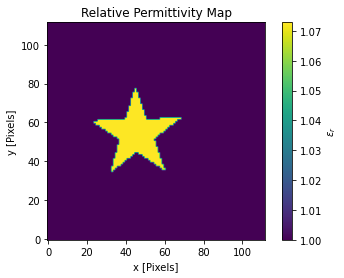
\includegraphics[width=0.4\textwidth]{./figuras/annex/02_zetas/output_2_0.png}}
			\subfloat[Recovered]{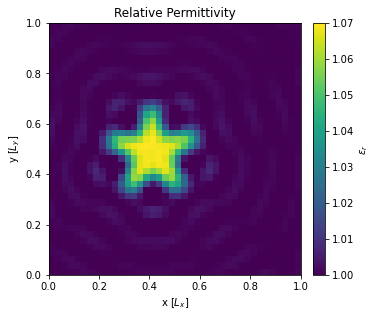
\includegraphics[width=0.4\textwidth]{./figuras/annex/02_zetas/output_4_0.png}}
			\caption{Example images for shape metrics.}
			\label{fig:annex:zetas:example}
		\end{figure}
		\begin{figure}[!htb]
			\centering
			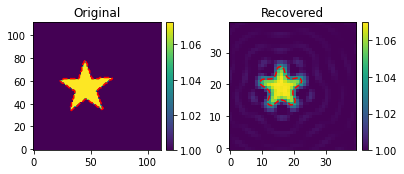
\includegraphics[width=.7\textwidth]{./figuras/annex/02_zetas/output_8_1.png}
			\caption{Contours of original and recovered images.}
			\label{fig:annex:zetas:contours}
		\end{figure}
		
		The main ideia is to calculate the difference area of the two contours. Of course, the area of one minus the area of the other would not work because the two forms might have equal areas but completely different forms. The following algorithm calculates the area of the difference:
		\begin{enumerate}
			\item Calculate the contours;
			\item Correct the scale of the recovered contour to be equivalent to the size of the original image;
			\item Center the image to isolate the object's position effect;
			\item Check which pixels of the image are on each of the objects;
			\item Separate those pixels that are in one of the objects and not in the other;
			\item Calculate the quantity and multiply by an area element considering the limits equal to 0 and 1.
		\end{enumerate}
		
		This algorithm is implemented in the following Python3 code: {\footnotesize
		\begin{lstlisting}[language=Python]
# Evaluate contourns
co = measure.find_contours(original, 1.0, fully_connected='high')
cr = measure.find_contours(recovered, threshold)

# Converting scale of recovered contourn
for i in range(len(cr)):
cr[i][:, 1] = original.shape[1]*cr[i][:, 1]/recovered.shape[1]
cr[i][:, 0] = original.shape[0]*cr[i][:, 0]/recovered.shape[0]

# Thresholding
masko = np.zeros(original.shape, dtype=bool)
maskr = np.zeros(recovered.shape, dtype=bool)
masko[original > 1] = True
maskr[recovered >= threshold] = True

# Evaluate centers
xo, yo = np.meshgrid(np.arange(0, original.shape[1]),
                     np.arange(0, original.shape[0]))
xr, yr = np.meshgrid(np.linspace(0, original.shape[1]-1, recovered.shape[1]),
                     np.linspace(0, original.shape[0]-1, recovered.shape[0]))
xco = np.sum(masko*xo)/np.sum(masko)
yco = np.sum(masko*yo)/np.sum(masko)
xcr = np.sum(maskr*xr)/np.sum(maskr)
ycr = np.sum(maskr*yr)/np.sum(maskr)

# Centralization
for i in range(len(co)):
co[i][:, 0] = co[i][:, 0]-yco+original.shape[0]/2
co[i][:, 1] = co[i][:, 1]-xco+original.shape[1]/2

# Centralization
for i in range(len(cr)):
cr[i][:, 0] = cr[i][:, 0]-ycr+original.shape[0]/2
cr[i][:, 1] = cr[i][:, 1]-xcr+original.shape[1]/2

# Verify points
masko = np.zeros(original.shape, dtype=bool)
counter = np.zeros(original.shape)
for i in range(len(co)):
maskt = measure.grid_points_in_poly(original.shape, co[i])
counter[maskt] += 1
masko[np.mod(counter, 2) == 1] = True

# Verify points
maskr = np.zeros(original.shape, dtype=bool)
counter = np.zeros(original.shape)
for i in range(len(cr)):
maskt = measure.grid_points_in_poly(original.shape, cr[i])
counter[maskt] += 1
maskr[np.mod(counter, 2) == 1] = True

# Xor operation
diff = np.logical_xor(masko, maskr)

# Area of the difference
zeta_s = np.sum(diff)/np.sum(masko)*100

# Figure
fig, axis = plt.subplots(ncols=3, figsize=[3*6.4,4.8])
fig.subplots_adjust(wspace=.5)
axis[0].imshow(masko, origin='lower')
axis[0].set_title('Original')
axis[1].imshow(maskr, origin='lower')
axis[1].set_title('Recovered')
axis[2].imshow(diff, origin='lower')
axis[2].set_title('Difference')

plt.show()
		\end{lstlisting}}
		
		This code yields results in \autoref{fig:annex:zetas:results}. The $\zeta_S$ measure in this case was 20.68\%.
		\begin{figure}[!htb]
			\centering
			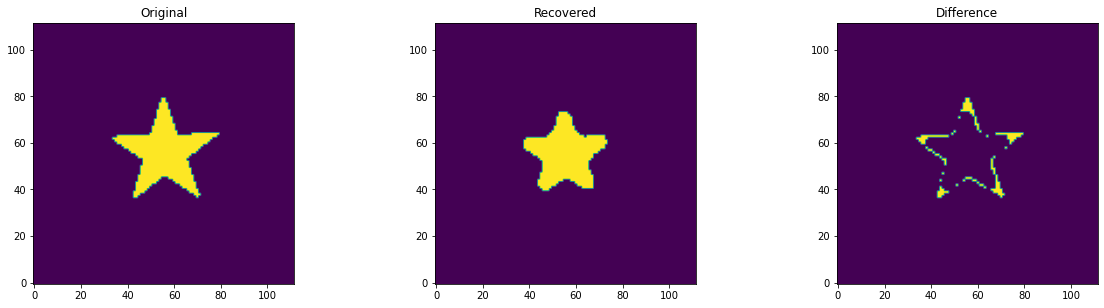
\includegraphics[width=\textwidth]{./figuras/annex/02_zetas/output_20_0.png}
			\caption{Original, recovered and difference area.}
			\label{fig:annex:zetas:results}
		\end{figure}
